\chapter{Metaheuristieken}
\begin{itemize}
    \item \textbf{Heuristieken} zijn vuistregels bij het zoeken naar een oplossing van een probleem.
    \item Garanderen niet dat er een oplossing gevonden wordt, maar versnelt wel de zoektocht ernaar.
\end{itemize}

\section{Combinatorische optimisatie}
\begin{itemize}
    \item Abstracte representatie van de problemen nodig. 
    \begin{itemize}
        \item Het zijn \textbf{optimisatie}-problemen.
        \item Voor een verzameling $\mathcal{S}$ moet hieruit de beste gekozen worden.
        \item De verzameling $\mathcal{S}$ is een eindige verzameling van strings over een eindig alfabet.
        \item Het beste individu wordt bepaald door een evaluatiefunctie $f$.
        \item De beste waarde komt overeen met de kleinste waarde voor $f$.
    \end{itemize}
    \item Voorbeeld bij het Travelling Salesman probleem:
    \begin{itemize}
        \item Het alfabet is hier de verzameling verbindingen.
        \item De verzameling $\mathcal{S}$ bestaat uit een reeks verbindingen zo dat elke verbinding vertrekt uit het eindpunt van de vorige en zo dat alle steden bezocht worden.
        \item Het beste individu is die met de kleinste lengte.
    \end{itemize}

    \item Vaak zijn alle strings in $\mathcal{S}$ even lang.
    \begin{itemize}
        \item Elementen van $\mathcal{S}$ kunnen dan beschreven worden door variabelen.
        \item Elke letter $s \in \mathcal{S}$ geeft de waarde aan van een variabele.
        \item Voorbeeld bij het lessenroosterprobleem:
        \begin{itemize}
            \item Er zijn een aantal lessen, een aantal docenten, een aantal klaslokalen, een aantal mogelijke tijdsslots en een aantal groepen studenten.
            \item Er moet een lessenrooster opgesteld worden zodanig dat er minimale negatieve elementen zijn (springuren, onevenwichtige verdelingen van de studenten, ...).
            \item Elke string van $\mathcal{S}$ is even lang en beschrijft e en lessenrooster zonder conflicten door aan elke les een lokaal en een tijdsslot toe te kennen.
            \item $\mathcal{S}$ heeft twee letters: de eerste duidt de tijdsslot aan en de tweede het lokaal.
        \end{itemize}
    \end{itemize}
    \item In principe zijn zulke problemen oplosbaar met backtracking.
    \item Maar voor problemen die te groot zijn voor backtracking, zijn metaheuristieken toch nodig.
    \item Er wordt daarom eerst een steekproef genomen uit de totale verzameling $\mathcal{S}$ en voor elk individu wordt de $f-$waarde berekend.
    \item Het individu met de beste $f-$waarde wordt altijd bijgehouden.
    \item Het zoeken stop na een bepaald criterium, zoals bijvoorbeeld een tijdslimiet of als het gevonden individu reeds goed genoeg is.
    \item De verschillende metaheuristieken verschillen in de manier waarop individuen worden uitgekozen om te vergelijken.
    \item Elke metaheuristiek leent zich ertoe om lokale optimalisaties door te voeren.
\end{itemize}


\section{Vooronderstellingen}

\begin{itemize}
    \item Bij de keuze van methodieken moet er eerst nagegaan worden of het probleem aan een aantal voorwaarden voldoet. Het ontbreken van een bepaalde voorwaarde kan bijvoorbeeld een metaheuristiek uitsluiten. Er zijn \textbf{vier} gebieden waarin onderscheidt tussen de verschillende optimisatietechnieken gemaakt kan worden.
    \begin{enumerate}
        \item \textbf{Het moet zinvol zijn om op zoek te gaan naar betere individuen in de buurt van een gegeven individu.} Het kan zijn dat we een individu van de grond af opbouwen (zeker bij het eerste individu), maar er moeten ook pogingen ondernomen worden om een reeds bestaand individu te verbeteren.
        \item \textbf{Soms is het niet zinvol om bij het opbouwen van een nieuw individu van $\mathcal{S}$ uit te gaan van reeds bekende individuen.} Een nieuw individu van de grond opbouwen kan op twee manieren:
        \begin{enumerate}
            \item Het individu wordt opgebouwd uit componenten. Deze componenten komen overeen met letters van de strings in $\mathcal{S}$. Dit gebeurt at random, eventueel met een bepaalde heuristiek die zeer slechte individuen uitsluit.
            \item Het individu wordt rechtstreeks aangemaakt.
        \end{enumerate}

        In het travelling salesman probleem kan een individu beschouwd worden als een pad in een graaf. Via de eerste methode is het pad leeg en worden verbindingen toegevoegd. In het tweede geval is het individu een permutatie van de verzameling verbindingen.

        \item \textbf{Een heuristiek moet aangeven dat een bepaalde keuze beter is dan de andere.} Bij het opbouwen van de componenten van een individu zijn sommige keuzes niet meer zinvol. Die mogen dan zeker niet meer gekozen worden. Er zijn twee mogelijkheden om dit te realiseren.
        \begin{enumerate}
            \item \textbf{Shortlisting.} Eerst worden de beste kandidaten geselecteerd met behulp van een bepaalde cutoff. Daarna wordt hieruit gekozen met gelijke waarschijnlijkheid.
            \item \textbf{Gewogen keuze.} Elke mogelijkheid krijgt een een gewicht $w_i$. De kans $p(i)$ dat $i$ gekozen wordt is dan
            $$p(i) = \frac{w_i}{\sum_j w_j}$$
        \end{enumerate}

        \item \textbf{Er zijn drie fundamentele methoden om een nieuw individu $\mathcal{S}$ te kiezen uitgaande van andere individuen.}
        \begin{enumerate}
            \item Kleine wijzigingen aanbrengen in een reeds bekeken individu $s$ van $\mathcal{S}$.
            \item Kruisen van twee bekeken individuen. 
            \item Het vermengen van een grote hoeveelheid al bekeken individuen.
        \end{enumerate}
    \end{enumerate}
\end{itemize}


\section{Lokaal versus globaal zoeken}
\begin{itemize}
    \item Bij het opbouwen van nieuwe  individuen van $\mathcal{S}$ moet het zinvol zijn om een individu van $\mathcal{S}$ te verbeteren door kleine aanpassingen.
    \item Een kleine aanpassing hangt af van het probleem.
    \begin{itemize}
        \item Voor elke $s \in \mathcal{S}$ is er een \textbf{omgeving} $\mathcal{N}(s)$: de omgeving van $s$ die bestaat uit $s$ zelf en alle strings uit $\mathcal{S}$ die door één kleine wijziging uit $s$ bekomen kunnen worden.
    \end{itemize}  
    \item Een goed individu kan zeker in een slecht individu omgevormd worden, maar vaker blijft het een goed individu.
    \item Lokale verbeteringen kunnen iteratief toegepast worden:
    \begin{itemize}
        \item Beginnend van een individu $s_0 \in \mathcal{S}$
        \item Genereer een rij van individuen $s_1, \cdots , s_n \in \mathcal{S}$.
        \item Hierbij geldt dat voor alle $i = 0, \cdots, n-1, s-i+1 \in \mathcal{N}(s_i)$ en $f(s_{i + 1}) < f(s_i)$. 
        \item Dit eindigt met een lokaal minimum, een individu $s_n$ zodat $\forall s \in \mathcal{N}(s_n): f(s) \geq f(s_n)$.
    \end{itemize}
    \item Het vinden van zo een rij heet \textbf{lokale optimisatie}.
    \item Zo een rij vinden kan op meerdere manieren:
    \begin{enumerate}
        \item \textbf{Steepest hill climbing.} (of steepest slope descending)

        Soms is het gemakkelijk om een lokaal minimum te vinden omdat $\mathcal{N}(s)$ weinig individuen bevat.

        \item \textbf{Randomisatie.}

        Veranderingen worden random gekozen.
    \end{enumerate}

    \item Er kunnen veel lokale minima zijn in $\mathcal{S}$, elk met een verschillende $f-$waarde.
    \item Er moet een manier zijn om te ontsnappen aan een lokaal minimum $\rightarrow$ \textbf{exploratie}.
    \begin{enumerate}
        \item Exploratie door helemaal opnieuw te beginnen.
        \item Exploratie door grotere wijzigingen aan te brengen aan gekende individuen.
    \end{enumerate}
\end{itemize}

\section{Methodes zonder recombinatie}
\begin{itemize}
    \item Random zoeken kan efficiënter gemaakt worden.
    \begin{enumerate}
        \item Lokaal zoeken verbetert vaak random aangemaakt individuen.
        \item Heuristieken gebruiken om het aanmaken van de individuen te sturen.
    \end{enumerate}
\end{itemize}

\subsection{Simulated Annealing}
\begin{itemize}
    \item Tijdens lokale optimisatie maakt het gebruik van een kans op een individu $s'$, ook al is $s'$ slechter dan $s$.
    \item De kans hangt af van:
    \begin{itemize}
        \item De evaluatiewaarden $f(s)$ en $f(s')$.
        \item Een 'temperatuur' $T$.
    \end{itemize}
    \item De kans wordt groter indien $T$ kleiner is of indien $f(s') - f(s)$ kleiner is (Boltzmanndistributie).
    $$\rho(T, f(s'), f(s)) = \exp\bigg(\frac{f(s') - f(s)}{T}\bigg)$$
    \item $T$ wordt vrij hoog gekozen, zodat exploratie bevorderd wordt en wordt iteratief gedaald tot bijna nul.
    \item Dit algoritme vindt zeer waarschijnlijk een globaal optimum als er een $\Gamma > 0$ bestaat waarvoor
    $$\sum_{k = 1}^{\infty} \exp\bigg(\frac{-\Gamma}{T_k}\bigg) = \infty $$
\end{itemize}

\subsection{Tabu Search}
\begin{itemize}
    \item Houdt een taboelijst bij: een lijst van al gecontroleerde individuen die niet opnieuw mogen bezocht worden.
    \item Alle gecontroleerde individuen bijhouden is niet efficiënt, daarom maar een beperkt aantal.
    \item De lijst bevorderd exploratie: bij een grote lijst zal een nieuwe individu veel verder in de omgeving $\mathcal{N}(s)$ liggen.
    \item De taboelijst kan ook eigenschappen bijhouden en geen individuen.
\end{itemize}

\section{Genetische algoritmen}
\begin{itemize}
    \item Meeste genetische algoritmen maken gebruik van \textbf{kruising}.
    \item Kruising is het combineren van twee individuen.
    \item Enkel zinvol als een kruising een beter individu \textit{kan} opleveren.
    \item Kruising combineerd meestal de componenten van beide individuen die goed kunnen zijn.
    \item Handig als één van de individuen een slechte $f-$waarde heeft.
    \item Twee manieren om te kruisen:
    \begin{enumerate}
        \item \textbf{Gerichte kruising.}
        
        Enkel haalbaar als er een algemeen idee is van de structuur van individuen.
        \item \textbf{Blinde kruising.}

        Gerandomiseerde kruising van componenten.

    \end{enumerate}
    \item Er is een \textbf{populatie nodig}.
    \item Het doel is dan om de algemen populatie te verbeteren.
    \item Men spreekt van \textbf{generaties}. De overstap van een generatie naar een andere gebeurt als volgt (figuur \ref{fig:genetisch_algoritme}):
    \begin{figure}[ht]
        \centering
        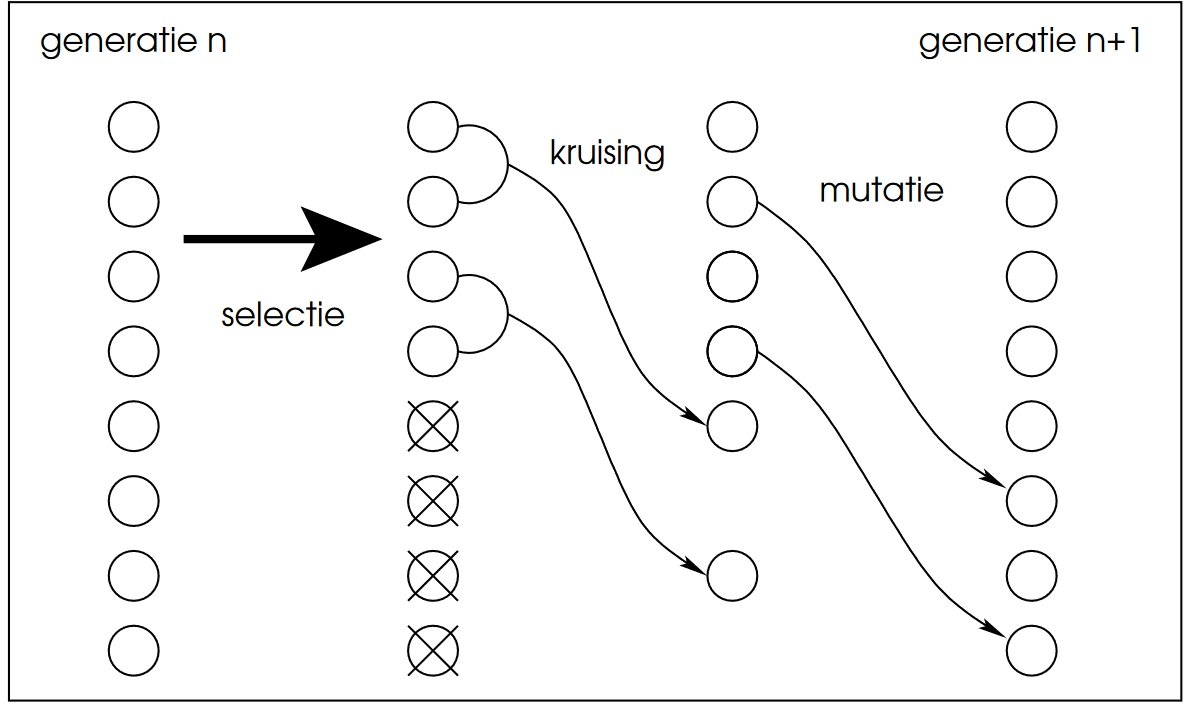
\includegraphics[width=0.5\textwidth]{genetisch_algoritme}
        \caption{Overgang naar een volgende generatie.}
        \label{fig:genetisch_algoritme}
    \end{figure}
    \begin{enumerate}
        \item De populatie wordt uitgedund zodat enkel de beste individuen overblijven.
        \item De populatie wordt terug aangevuld op basis van de overblijvende individuen door kruising en mutatie.
    \end{enumerate}

    \item Twee verfijningen:
    \begin{itemize}
        \item Twee componenten kunnen elkaar positief beïnvloeden. Het is dan interessant om deze componenten bij elkaar te houden. Dit kan ingebouwd worden bij gerichte kruising. Er kan ook een maat voor gelijkaardigheid ingevoerd worden.
        \item Kruising moet niet enkel zorgen voor betere individuen, maar ook voor diversificatie en zo voor exploratie. Zo voert men \textbf{niching} in, dat de fitheid van individuen verminderd naarmate er meer gelijkaardige individuen in de populatie zitten.
    \end{itemize}

\end{itemize}


\section{Vermenging}
\begin{itemize}
    \item Niet twee individuen kruisen, maar de globale eigenschappen van de hele populatie wordt in beschouwing genomen.
    \begin{enumerate}
        \item \textbf{Componentniveau.} Hierbij gaat men ervan uit dat het succes van een individu afhangt van de individuele componenten die ze bevat.
        \item \textbf{Combinatieniveau.} Hierbij gaat men ervan uit dat het succes van een individu afhangt van de combinatie van componenten die ze bevat.
    \end{enumerate}
\end{itemize}

\subsection{Recombinatie op componentniveau}
\begin{itemize}

    \item Er wordt een $f-$waarde toegekend niet enkel aan de individuen, maar ook aan de componenten zelf.
    \item Het construeren van een nieuwe populatie gebeurt pseudorandom waarbij gewicht $w_i$ van component $i$ dient als gewicht voor de gewogen keuze.
    \item De gewogen random keuze kiest uit een verzameling $\mathcal{V}$ van componenten een component $i$ met waarschijnlijkheid

    $$p(i) = \frac{w_i}{\sum_{j \in V}w_j}$$

    \item Twee belangrijke metaheuristieken die gebruik maken van dit soort recombinatie. Ze verschillen in de manier waarop gewichten aan componenten toegekend worden.
    \begin{itemize}
        \item \textbf{Gene Pool Recombiniation (GPR)}.
        
        Elk component krijgt een gewicht evenredig met het aantal individuen in de overblijvende populatie die het component bevatten. Het gewicht van een component is dan enkel afhankelijk van de vorige generatie.
        \item \textbf{Ant Colony Optimisation (ACO)}.

        Elke $s$ krijgt eerst een kwaliteitswaarde $F(s)$, die groter is naarmate $f(s)$ kleiner is. Een nieuw gewicht voor een component $i$ is dan
        $$w_i = (1 - \rho)w_i + \sum_{s\hbox{ bevat } i} F(s)$$

        met $\rho$ de vergeetfactor. Het gewicht van meerdere generaties zal invloed hebben op het huidige gewicht.

        
    \end{itemize}
\end{itemize}

\subsection{Recombinatie op combinatieniveau}
\begin{itemize}
    \item Er zijn twee voorwaarden om dergerlijke methoden te gebruiken:
    \begin{enumerate}
        \item Opeenvolgende letters in het individu moeten een sterk onderling verband vertonen.
        \item Een deelstring van een goed individu gebruiken in een ander individu verhoogt de kans dat het andere individu ook goed is.
    \end{enumerate}
    \item De componenten van de individuen worden de knopen van een ongerichte gewogen graaf.
    \item Als twee componenten samen kunnen voorkomen is er een verbinding tussen de overeenkomstige knopen in de graaf.
    \item Er zijn nu een aantal \textbf{agents} die proberen een individu uit $\mathcal{S}$ te construeren. Dit wordt voorgesteld door een pad in de graaf.
    \begin{enumerate}
        \item Op een bepaald punt bepaalt de agent of het pad een individu definieert. Zo ja dan stopt het.
        \item Anders worden de componenten bepaalt die nog in aanmerking komen.
        \item Als er geen mogelijkheden zijn wordt er gestopt, anders wordt er een gewogen keuze gemaakt tussen de verbindinge.
    \end{enumerate}
    \item Nadat elke agent geprobeerd heeft om een individu te construeren, worden de gewichten aangepast.
    \item Elke agent die een individu $s$ heeft gevonden, past het gewicht aan van elke verbinding dat het gebruikt heeft met $F(s)$ 
    $$\tau_{ij} = (1 - \rho)\tau_{ij} + \sum_{s \in A_{ij}} F(s)$$
    
    Hierbij is $A_{ij}$ de verzameling individuen die verbinding $v_{ij}$ gebruikt hebben.

    \item Meestal zijn alle $\tau_{ij}$ eerst gelijk, maar andere beginwaarden zijn ook mogelijk.
\end{itemize}